\section{Methods}
\label{sec:methods}

Talk about:
\begin{itemize}
\item difference wrt to Barett-Jolley 2011 in terms of channels chosen
\item availability of code
\item the fact that we are introducing a ``comprehensive model'' but
  will only focus on some channels
\end{itemize}

\subsection{Model Development}
\label{sec:model-development}

In this discourse, we focus our attention on a single chondrocyte cell
residing in deep regions of cartilage. This cartilage environment is
modelled simply by (fixed) external concentrations \Nao, \Ko, \Cao,
and \Ho. Values for these concentrations are chosen within
physiologically-relevant ranges (see
Table~\ref{table:external-concentrations}). We are interested in
studying the behaviour of cell under this environment, in particular
looking at how the flux of these ions through membrane channels
changes their internal concentrations over time and how this changes
the cell's membrane potential. The channels under consideration are
illustrated in Figure~\ref{fig:chondrocyte-model}.

\begin{table}[ht]
\begin{centering}
\begin{tabular}{r c c c c}
\hline\hline
             & \Nao (mM) & \Ko (mM) & \Cao (mM) & pH\\
\hline
Surface zone & 240--270  & 7--9     & 6--9      & 7.1--7.3\\
Deep zone    & 300--350  & 9--12    & 14--20    & $\sim$6.9\\
\hline
\hline
\end{tabular}
\caption{Experimental ranges of external concentrations
  \citep{Halletal1996}.}
\label{table:external-concentrations}
\end{centering}
\end{table}

\begin{figure}[ht]
  \centering
  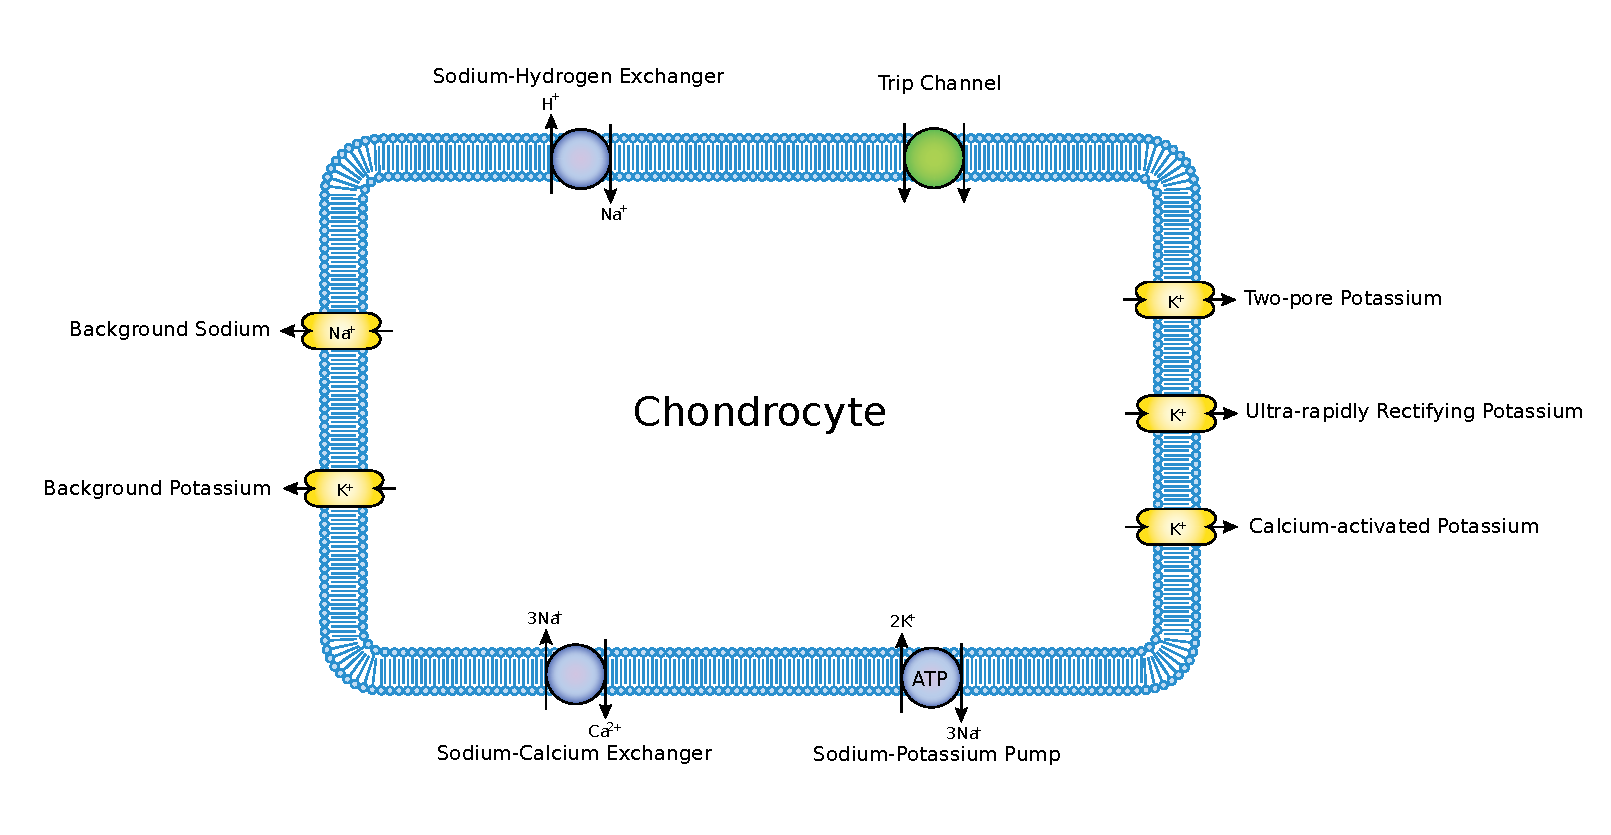
\includegraphics[width=\textwidth]
  {../images/pdf/chondrocyte-model-cellml}
  \caption{An illustration of the model.}
  \label{fig:chondrocyte-model}
\end{figure}

In order to simplify the treatment, we assume that there are no
spatial variations in these quantities of interest, allowing us to
model the cell as the following set of ordinary differential equations
(ODEs) in time.

\begin{equation}
  \frac{d}{dt}
  \left(
    \begin{array}{c}
      V_{\rm m}\\
      \left[Na^{+}\right]_{i}\\
      \left[\rm K^{+}\right]_{i}\\
      \left[\rm Ca^{2+}\right]_{i}\\
      \left[\rm H^{+}\right]_{i}\\
      a_{\rm ur}\\
      i_{\rm ur}\\
    \end{array}
  \right)  = \left(
    \begin{array}{c}
        (-I_{i} + I_{\rm stim})/{C_{\rm m}}\\
      - (I_{\rm Na_{b}} + 3\, I_{\rm NaK} + 3\, I_{\rm NaCa} - I_{\rm
        NaH})/(v_{i}\, F)\\
      - (I_{\rm K_{b}} - 2\, I_{\rm NaK} + I_{\rm K_{ur}} + I_{\rm
        K_{2\, pore}} + I_{\rm K_{Ca-act}} + I_{\rm K_{ATP}})/(v_{i}\,
      F)\\
        (I_{\rm NaCa})/(v_{i}\, F)\\
      - (I_{\rm NaH})/(v_{i}\, F)\\
      (a_{{\rm ur}_{\infty}} - a_{\rm ur})/\tau_{a_{\rm ur}}\\
      (i_{{\rm ur}_{\infty}} - i_{\rm ur})/\tau_{i_{\rm ur}}\\
    \end{array}
  \right)
\end{equation}

\noindent where,

\begin{displaymath}
    \begin{split}
      I_{i} =
      & \phantom{+\,} \underbrace{I_{\rm Na_b} + I_{\rm K_b}}_{\rm
        Background\, currents}\\
      & +\, \underbrace{I_{\rm NaK} + I_{\rm NaCa} + I_{\rm NaH}}_{\rm
        Pumps\, and\, exchangers}\\
      & +\, \underbrace{I_{\rm K_{ur}} + I_{\rm K_{2\, pore}} + I_{\rm
          K_{Ca-act}} + I_{\rm K_{ATP}}}_{\rm Potassium\, channels}\\
      & +\, \underbrace{I_{\rm ASIC} + I_{\rm TRP1} + I_{\rm TRP2} +
        I_{\rm stim}}_{\rm Other\, currents}
    \end{split}
\end{displaymath}

This ODE system is solved for the primary vector of unknowns: $V_{\rm
m}$, $Na_{\rm i}$, $K_{\rm i}$, $Ca_{\rm i}$, $H_{\rm i}$, $a_{\rm
ur}$, $i_{\rm ur}$.

\subsection{Background Currents}
\label{sec:background-currents}

Background Sodium Current (Hodgkin Huxley?):
\begin{equation}
  \begin{split}
    I_{\rm Na_b} & = \bar{g}_{\rm Na_b} (V_{\rm m} - E_{\rm Na})\\
    E_{\rm Na} & =  \frac{R T}{z_{\rm Na} F}
    \ln\left(\frac{\left[Na^{+}\right]_{o}}
      {\left[Na^{+}\right]_{i}}\right)
  \end{split}
\end{equation}

Background Potassium Current (Hodgkin Huxley?):
\begin{equation}
  \begin{split}
    I_{\rm K_b} & = \bar{g}_{\rm K_b} (V_{\rm m} - E_{\rm K})\\
    E_{\rm K} & =  \frac{R T}{z_{\rm K} F}
    \ln\left(\frac{\left[K^{+}\right]_{o}}
      {\left[K^{+}\right]_{i}}\right)
  \end{split}
\end{equation}

\subsection{Pumps and exchangers}
\label{sec:pumps-and-exchangers}

Sodium Potassium Pump \citep[Table 12, pp. 77]{Nygrenetal1998}:
\begin{equation}
  I_{\rm NaK} =
  \bar{I}_{\rm NaK} \left( \frac{[\rm K^{+}]_{\rm o}}{[\rm K^{+}]_{\rm o} +
    k_{\rm NaK_{K}}} \right) \left(\frac{[\rm Na^{+}]^{1.5}_{\rm i}}{[\rm
    Na^{+}]^{1.5}_{\rm i} + k^{1.5}_{\rm NaK_{Na}}}\right) \left( \frac{V + 150}{V +
    200} \right)
\end{equation}

Sodium Calcium Exchanger \citep[Table 13, pp. 77]{Nygrenetal1998}:
\begin{equation}
  I_{\rm NaCa} = k_{\rm NaCa} \frac{[\rm Na^{+}]^{3}_{i}[\rm
    Ca^{2+}]_{o} \exp(\frac{\gamma V F}{R T}) - [\rm
    Na^{+}]^{3}_{o}[\rm Ca^{2+}]_{i} \exp(\frac{(\gamma - 1.0) V F}{R
      T})} {1.0 + d_{\rm NaCa}([\rm Na^{+}]^{3}_{o}[\rm Ca^{2+}]_{i} +
    [\rm Na^{+}]^{3}_{i}[\rm Ca^{2+}]_{o})}
\end{equation}

Sodium Hydrogen Exchanger \citep[Eq. 2, pp. 2675]{Chaetal2009}
\begin{equation}
  \begin{split}
    I_{{\rm NaH}_{\rm mod}} & = \frac{1}{1 + (K_{\rm i}^{n_{\rm
          H}}/[{\rm H}^{+}]_{\rm i}^{n_{\rm H}})}\\
    t_{1} & = \frac{k_{1}^{+} [{\rm Na}^{+}]_{\rm o}/K_{\rm Na}^{\rm
        o}} {(1 + [{\rm Na}^{+}]_{\rm o}/K_{\rm Na}^{\rm o} + [{\rm
        H}^{+}]_{\rm o} /K_{\rm H}^{\rm o})}\\
    t_{2} & = \frac{k_{2}^{+} [{\rm H}^{+}]_{\rm i}/K_{\rm H}^{\rm i}}
    {(1 + [{\rm Na}^{+}]_{\rm i}/K_{\rm Na}^{\rm i} + [{\rm
        H}^{+}]_{\rm i}/K_{\rm H}^{\rm i})}\\
    t_{3} & = \frac{k_{1}^{-} [{\rm Na}^{+}]_{\rm i}/K_{\rm Na}^{\rm
        i}} {(1 + [{\rm Na}^{+}]_{\rm i}/K_{\rm Na}^{\rm i} + [{\rm
        H}^{+}]_{\rm i} /K_{\rm H}^{\rm i})}\\
    t_{4} & = \frac{k_{2}^{-} [{\rm H}^{+}]_{\rm o}/K_{\rm H}^{\rm
        o}} {(1 + [{\rm Na}^{+}]_{\rm o}/K_{\rm Na}^{\rm o} + [{\rm
        H}^{+}]_{\rm o} /K_{\rm H}^{\rm o})}\\
    I_{{\rm NaH}_{\rm exch}} & = \frac{(t_1 t_2 - t_3 t_4)}
    {(t_1 + t_2 + t_3 + t_4)}\\
    I_{\rm NaH} & = N_{\rm NaH} I_{\rm NaH_{\rm mod}}
    I_{\rm NaH_{\rm exch}}
  \end{split}
\end{equation}

\subsection{Potassium channels}
\label{sec:potassium-channels}

Ultra-rapidly rectifying potassium channel \citep{Maleckaretal2009}:
\begin{equation}
  \begin{split}
    I_{\rm K_{\rm ur}} & = g_{\rm K_{\rm ur}}\, a_{\rm ur}\, i_{\rm
      ur}\, (V - E_{\rm K})\\
    E_{\rm K} & =  \frac{R T}{z_{\rm K} F}
    \ln\left(\frac{\left[K^{+}\right]_{o}}
      {\left[K^{+}\right]_{i}}\right)\\
    a_{{\rm ur}_{\infty}} & = \frac{1}{1 + \exp(-(V_{\rm m} +
      6.0)/8.6)}\\
    i_{{\rm ur}_{\infty}} & = \frac{1}{1 + \exp(-(V_{\rm m} +
      7.5)/10.0)) + 0.7}\\
    \tau_{a_{\rm ur}} & = \frac{0.009}{1 + \exp((V + 5.0)/12.0)} +
    0.0005\\
    \tau_{i_{\rm ur}} & = \frac{0.5}{1 + \exp((V +60.0)/20.0)} +
    6\\
  \end{split}
\end{equation}

Two-pore potassium channel \citep{UNKNOWN}:
\begin{equation}
 I_{\rm K_{2\, pore}} = P_{\rm K}\, \frac{z_{\rm K}^2\, V\, F^{2}}{R\,
   T}\, \frac{({\left[K^{+}\right]_{i}} - {\left[K^{+}\right]_{o}}\,
 exp(\frac{-z_{\rm K}\, V\, F}{R\, T}))}{(1 - \exp(-z_K\, V\, F/(R\,
 T))}
\end{equation}

Calcium-activated potassium channel \citep{Horriganetal2002}:
\begin{equation}
  \begin{split}
    kTe & = 23.54\, (T/273)\\
    L_v & = L0\, \exp((V\, Z_L)/kTe)\\
    J_v & = \exp(((V - Vh_j)\, Z_j)/kTe)\\
    K & = Ca_i/KDc\\
    P_0 & = \frac{L_v\, (1+K\, C+J_v\, D+J_v\, K\, C\, D\, E)^4}
    {L_v\, (1+K\, C+J_v\, D+J_v\, K\, C\, D\, E)^4 +
      (1+J_v+K+J_v\, K\, E)^4}\\
    E_{\rm K} & =  \frac{R T}{z_{\rm K} F}
    \ln\left(\frac{\left[K^{+}\right]_{o}}
      {\left[K^{+}\right]_{i}}\right)\\
    I_{\rm K_{Ca-act}} & = N_{\rm K_{Ca-act}}\, P_0\, G_{\rm max}\, (V -
    E_{\rm K})
  \end{split}
\end{equation}

Potassium pump \citep{UNKNOWN}:
\begin{equation}
  I_{\rm K_{ATP}} =
\end{equation}

\subsection{Other channels}
\label{sec:other-channels}

Voltage-activated hydrogen channel \citep{UNKNOWN}:
\begin{equation}
  I_{\rm ASIC} =
\end{equation}

Stretch-activated trip channel \citep{UNKNOWN}:
\begin{equation}
  I_{\rm TRP1} = \bar{g}_{\rm TRP1}\, (V_{\rm m} - E_{\rm ?})
\end{equation}

Osteo-arthritic trip channel \citep{UNKNOWN}:
\begin{equation}
  I_{\rm TRP2} = \bar{g}_{\rm TRP2}\, (V_{\rm m} - E_{\rm ?})
\end{equation}

External stimulation (matching experiments, e.g. cyclic stimulation):
\begin{equation}
I_{\rm stim} = \overline{I_{\rm stim}}\, {\rm square}(\frac{2 \pi\,
  t}{t_{\rm cycle}}, \frac{t_{\rm stim}}{t_{\rm cycle}})
\end{equation}

% \begin{sidewaystable}[ht]
% \begin{tabular}{r c l l}
% \hline\hline
% Current description & Notation & Functional form & Parameter values \\ [0.5ex]
% \hline
% Background sodium & $I_{\rm Na_b}$ & $\bar{g}_{\rm Na_b} (V_{\rm m} - E_{\rm Na})$ \cite{UNKNOWN}
%                           & $\bar{g}_{\rm Na_b} = $ \cite{UNKNOWN}, $E_{\rm Na} = $ \cite{UNKNOWN}\\
% Background potassium & $I_{\rm K_b}$ & $\bar{g}_{\rm K_b} (V_{\rm m} - E_{\rm K})$ \cite{UNKNOWN}
%                           & $\bar{g}_{\rm K_b} = $ \cite{UNKNOWN}, $E_{\rm K} = $ \cite{UNKNOWN}\\
% Sodium-potassium pump & $I_{\rm NaK}$ & $\bar{I}_{\rm NaK}
% \frac{[\rm K^{+}]_{\rm c}}{[\rm K^{+}]_{\rm c} + k_{\rm NaK_{K}}}
% \frac{[\rm Na^{+}]^{1.5}_{\rm i}}{[\rm Na^{+}]^{1.5}_{\rm i} + k^{1.5}_{\rm
%     NaK_{Na}}}
% \frac{V + 150}{V + 200}$\cite{Nygrenetal1998} & \cite{Nygrenetal1998}\\
% Sodium-calcium exchanger & $I_{\rm NaCa}$ & $k_{\rm NaCa}
% \frac{[\rm Na^{+}]^{3}_{i}[\rm Ca^{2+}]_{c} \exp(\frac{\gamma V F}{R T}) -
% [\rm Na^{+}]^{3}_{c}[\rm Ca^{2+}]_{i} \exp(\frac{(\gamma - 1.0) V F}{R T})}
% {1.0 + d_{\rm NaCa}([\rm Na^{+}]^{3}_{c}[\rm Ca^{2+}]_{i} + [\rm
%   Na^{+}]^{3}_{i}[\rm Ca^{2+}]_{c})}$
% \cite{Nygrenetal1998} & \cite{Nygrenetal1998}\\
% Sodium-hydrogen exchanger & $I_{\rm NaH}$ & \cite{UNKNOWN} & \cite{UNKNOWN}\\
% Ultra-rapidly rectifying potassium & $I_{\rm K_{ur}}$ & $g_{\rm
%   K_{ur}}\, a_{\rm ur}\, i_{\rm ur}\, (V_{\rm m} - E_{\rm K})$ \cite{Maleckaretal2009} & \cite{Maleckaretal2009}\\
% Two-pore potassium channel & $I_{\rm K_{2\, pore}}$ & \cite{UNKNOWN} & \cite{UNKNOWN}\\
% Calcium-activated potassium & $I_{\rm Ca_{act}K}$ & \cite{UNKNOWN} & \cite{UNKNOWN}\\
% Trip channel(s) & $I_{\rm TRP}$ & $\bar{g}_{\rm NaCa_{TRP}}\, (V_{\rm
%   m} - E_{\rm NaCa})$ \cite{UNKNOWN} & \cite{UNKNOWN}\\
% Applied stimulus & $ I_{\rm stim}$ & Mirroring experiments \cite{Clarketal2011} &  --- \\ [1ex]
% \hline
% \end{tabular}
% \caption{Details of the model}
% \label{table:chondrocyte-model-details}
% \end{sidewaystable}

% Local Variables:
% TeX-master: "chondrocyte-model"
% mode: latex
% mode: flyspell
% End:
